\documentclass[sigconf]{acmart}

% Course report scaffold based on the provided ACM Overleaf template.
% Keep the supplied document class and formatting settings unchanged.
\settopmatter{printacmref=false}
\renewcommand\footnotetextcopyrightpermission[1]{}
\pagestyle{plain}

\usepackage{booktabs}
\usepackage{graphicx}
\usepackage{tikz}
\usetikzlibrary{arrows.meta,positioning,shapes.geometric}

\title[Skill-Augmented Search Agent]{COMP5423 Group Project Report: Skill-Augmented Search Agent}

% TODO: Replace the four author placeholders with your group members' full names.
\author{Member 1}
\affiliation{%
  \institution{The Hong Kong Polytechnic University}
  \country{Hong Kong SAR}
}
\author{Member 2}
\affiliation{%
  \institution{The Hong Kong Polytechnic University}
  \country{Hong Kong SAR}
}
\author{Member 3}
\affiliation{%
  \institution{The Hong Kong Polytechnic University}
  \country{Hong Kong SAR}
}
\author{Member 4}
\affiliation{%
  \institution{The Hong Kong Polytechnic University}
  \country{Hong Kong SAR}
}
\renewcommand{\shortauthors}{COMP5423 Group}

\begin{document}

\begin{abstract}
% TODO (write after the system and experiments are complete):
% Summarize the task, the proposed system, retrieval and agent design, skill use,
% evaluation setup, key measured results, and main conclusion. Do not report
% unmeasured results. Keep this abstract concise (approximately 150--200 words).
[Write a concise summary of the project here.]
\end{abstract}

\keywords{Search Agents, Information Retrieval, Tool Use, Agent Skills, BrowseComp-Plus}

\maketitle

\section{Introduction}
% Explain the BrowseComp-Plus task, why multi-step search is challenging, and
% the project goals. State the main contributions of your implemented system.
[Describe the problem context, motivation, objectives, and contributions.]

\section{Task and Dataset}
\subsection{Task Definition}
% Describe the input question, fixed document collection, and expected answer.
% Explain that the system must run on the released validation/test files.
[Define the task and expected system input/output.]

\subsection{Dataset}
% Document the BrowseComp-Plus collection and the validation/test split actually used.
% Report dataset versions, preprocessing, and any exclusions, if applicable.
[Describe the corpus, validation set, test set, and preprocessing.]

\section{System Design}
\subsection{Architecture Overview}
% Explain the overall architecture and the role of each component.
[Describe the implemented components and how they communicate.]

\subsection{End-to-End Workflow}
% Replace or revise the scaffold below so it accurately reflects the final implementation.
\begin{figure}[t]
  \centering
  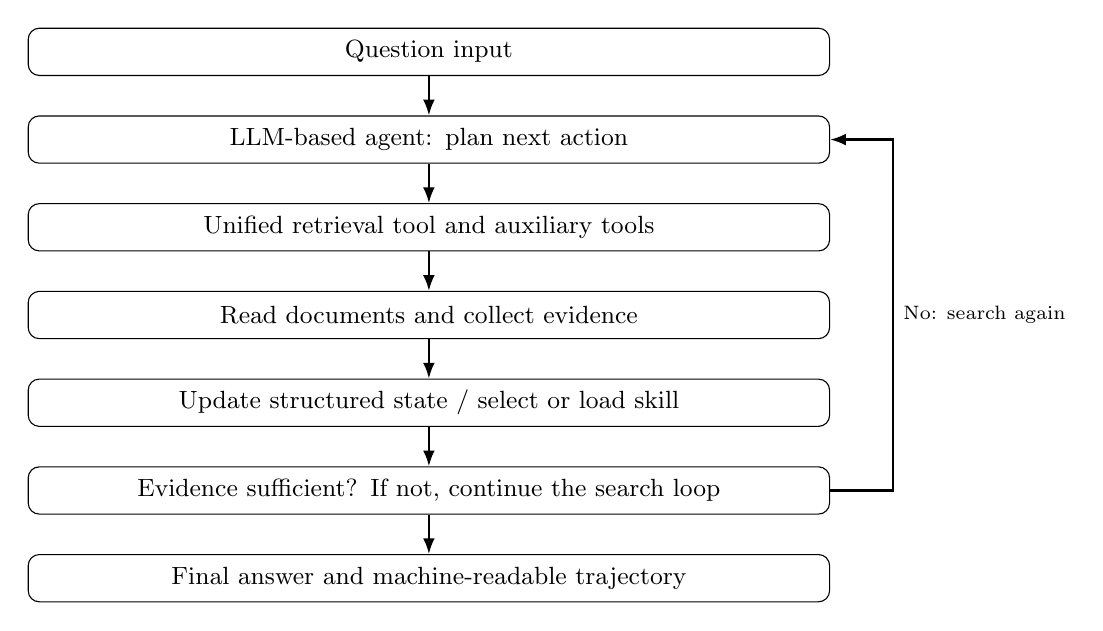
\begin{tikzpicture}[
    node distance=5mm,
    block/.style={draw, rounded corners, align=center, text width=0.82\linewidth,
                  minimum height=6mm, font=\small},
    arrow/.style={-{Latex[length=2mm]}, thick}
  ]
    \node[block] (q) {Question input};
    \node[block, below=of q] (agent) {LLM-based agent: plan next action};
    \node[block, below=of agent] (tool) {Unified retrieval tool and auxiliary tools};
    \node[block, below=of tool] (evidence) {Read documents and collect evidence};
    \node[block, below=of evidence] (state) {Update structured state / select or load skill};
    \node[block, below=of state] (decision) {Evidence sufficient? If not, continue the search loop};
    \node[block, below=of decision] (answer) {Final answer and machine-readable trajectory};
    \draw[arrow] (q) -- (agent);
    \draw[arrow] (agent) -- (tool);
    \draw[arrow] (tool) -- (evidence);
    \draw[arrow] (evidence) -- (state);
    \draw[arrow] (state) -- (decision);
    \draw[arrow] (decision) -- (answer);
    \draw[arrow] (decision.east) -- ++(8mm,0) |- node[pos=0.25,right,font=\scriptsize,align=left] {No: search again} (agent.east);
  \end{tikzpicture}
  \caption{Initial workflow scaffold. Revise the nodes and arrows to match the implemented system before submission.}
  \Description{A flowchart from question input through agent planning, retrieval and evidence collection, state and skill updates, a sufficiency decision, and final answer generation, with a loop for further search.}
  \label{fig:workflow}
\end{figure}
[Explain the workflow step by step and refer to Figure~\ref{fig:workflow}.]

\section{Retrieval and Tool Design}
\subsection{Retrieval Method}
% The assignment requires at least one retrieval family. Explain the method(s)
% actually implemented, indexing, ranking, score/fragment output, and any fusion.
[Describe the implemented retrieval approach and its design choices.]

\subsection{Auxiliary Tools}
% List each implemented agent-callable tool, with its name, purpose, inputs and outputs.
% The agent must have exactly one unified retrieval tool plus at least one auxiliary tool.
[Describe the auxiliary tools and their interfaces.]

\section{Search Agent}
\subsection{Tool-Use Loop}
% Explain how the specified DeepSeek-V4-Flash API is used, how actions are selected,
% tool calls are executed, observations are returned, and stopping is decided.
[Describe the implemented agent loop and stopping criteria.]

\subsection{Context and State Management}
% If implemented, describe visited-document tracking, evidence storage, query progress,
% deduplication, truncation, compression or summarization. Do not claim unimplemented features.
[Describe the state representation and context-control strategy.]

\section{Reusable Skills}
% The assignment requires at least one original Agent Skills-style skill in a directory
% containing SKILL.md with YAML frontmatter (name and description).
\subsection{Skill Structure}
[Describe the skill(s), their SKILL.md structure, and how the agent loads them at runtime.]

\subsection{Skill Selection and Execution}
% If two or more skills and automatic selection are implemented, explain the selection policy
% and provide examples showing different questions/states selecting different skills.
[Describe when each skill is selected and how it changes the agent's actions.]

\section{User Interface}
% Include actual screenshots of the terminal or web interface. Captions should explain
% how users submit a question and inspect answers, evidence, skills, and tool activity.
\begin{figure}[t]
  \centering
  \fbox{\parbox[c][35mm][c]{0.92\linewidth}{\centering
    TODO: Insert a screenshot of your implemented interface here.}}
  \caption{Placeholder for a screenshot of the implemented user interface. Replace before submission.}
  \Description{Placeholder box for a screenshot of the project interface.}
  \label{fig:ui}
\end{figure}
[Explain the user interaction flow and what evidence or execution details are displayed.]

\section{Experimental Setup}
\subsection{Evaluation Protocol}
% Specify which released split is used, number of questions, API/model configuration,
% repeated runs (if any), and the evaluation script.
[Describe the reproducible evaluation setup.]

\subsection{System Configurations}
% Define the variants you actually compare, e.g. retrieval choices, skill on/off,
% iteration on/off, or context-management variants. Do not include experiments not run.
[Describe the system configurations evaluated.]

\subsection{Metrics}
% The assignment specifies normalized exact match (EM), total tool calls, and total tokens.
% State the exact calculation and any additional metrics used.
[Define the metrics and evaluation procedure.]

\section{Results and Analysis}
% Replace the example table with measured results. Do not fabricate numbers.
\begin{table}[t]
  \centering
  \caption{Experimental results (fill in with measured values).}
  \label{tab:results}
  \begin{tabular}{lrrr}
    \toprule
    Configuration & EM (\%) & Tool calls & Tokens \\
    \midrule
    Baseline & -- & -- & -- \\
    Variant 1 & -- & -- & -- \\
    Variant 2 & -- & -- & -- \\
    \bottomrule
  \end{tabular}
\end{table}
[Report the measured results and analyze the effects of each configuration. Explain failures,
trade-offs, and representative cases. Remove unused rows and placeholders.]

\section{Discussion and Limitations}
% Discuss what worked, what did not, error patterns, cost/latency trade-offs, and limitations.
[Discuss limitations and lessons learned, grounded in your experiments.]

\section{Conclusion and Future Work}
[Summarize the implemented system and measured findings, then identify realistic next steps.]

% Optional section; keep only if there are real experiments or features to report.
\section{Additional Exploration (Optional)}
[Describe additional experiments, features, or optimizations if conducted; otherwise remove this section.]

%% COMPULSORY: retain and complete the provided contribution and declaration section.
\section*{CONTRIBUTION AND DECLARATION}

\subsection*{Contribution}
% TODO: Replace Member 1--4 with full names and describe actual contributions.
% Percentages must sum to exactly 100\%.
\begin{itemize}
    \item Member 1 (25\%): [Describe actual contribution.]
    \item Member 2 (25\%): [Describe actual contribution.]
    \item Member 3 (25\%): [Describe actual contribution.]
    \item Member 4 (25\%): [Describe actual contribution.]
\end{itemize}

\subsection*{Declaration}
We, the signed members of Group [X], hereby make the following declarations:
\begin{itemize}
    \item We confirm that the work presented in this project is the original result of our collective efforts, except where explicitly acknowledged through proper citation.
    \item We guarantee the authenticity of all data, the accuracy of all analyses, and the integrity of the results presented herein. We affirm that the work has been conducted in accordance with accepted academic principles of the university.
    \item We have collectively reviewed and critically evaluated all materials submitted for this project, acknowledge and agree with the contribution distribution stated above, and approve this final version of submission.
    \item We understand and acknowledge that academic misconduct, including plagiarism, fabrication, falsification, or other violations of academic integrity, may be subject to disciplinary action in line with university policies.
\end{itemize}

By signing below, each member confirms their consent to the statements above.

\begin{center}
\begin{tabular}{cccc}
\rule{0.20\linewidth}{0.4pt} &
\rule{0.20\linewidth}{0.4pt} &
\rule{0.20\linewidth}{0.4pt} &
\rule{0.20\linewidth}{0.4pt} \\
Member 1 & Member 2 & Member 3 & Member 4 \\
Signature & Signature & Signature & Signature
\end{tabular}
\end{center}


\bibliographystyle{ACM-Reference-Format}
\bibliography{references}
This report uses LaTeX for document preparation \cite{lamport1986latex}.
\end{document}
